\documentclass[12pt, spanish, pdftex]{UC3M_document}

%%%%% Preamble %%%%%
\author{Jorge Rodríguez Fraile}
\authorstwotrue
\authorsuptothree{Jorge Rodríguez Fraile}{100405951}{Grupo 83}{}{}{}{}{}{}


%%%%% Basic data about the document (Degree, subject, title, campus, page number custom text) %%%%%
\documentdata{Grado en Ingeniería Informática}{Algoritmos Genéticos y Evolutivos}{Práctica 1 \\ Optimización de Sensores en Smart Cities}{Leganés}{}

%%%%% Page style %%%%%
\header
\footer
\pagestyle{fancy}

\begin{document}
%%%%% Page title %%%%%
\begin{titlepage}
	\centeredtitle{img/LogoUC3M.png}{\studyname}{Curso 2021-2022}{\subjectname}{\documenttitle}
	
	\begin{table}[b]
		\centering
		\begin{tabular}{ cccc }
			\large Jorge Rodríguez Fraile & \large 100405951 & \large Grupo 83 & \href{mailto:100405951@alumnos.uc3m.es}{\large 100405951@alumnos.uc3m.es} \\
			                              &                  &                 &                                                                           \\
			                              &                  &                 &                                                                           \\
		\end{tabular}
	\end{table}
	
\end{titlepage}

\newpage

%%%%% Index %%%%%
\begin{spacing}{0.5}
	% \shipout\null                   % Blank page before index (after title page)
	\hypersetup{linkcolor=black}    % References/links on the index will remain black color
	\tableofcontents\newpage        % Index of the document
	\listoffigures\newpage          % Index of pictures
	\listoftables\newpage           % Index of tables
\end{spacing}


%%%%% DOCUMENT CONTENT %%%%%
\section{Introducción}
En los últimos años ha aumentado mucho el interés por las Ciudades Inteligentes o Smart Cities, desde que la mayoría de la población se encuentran en ciudades. La aplicación de la tecnología en las ciudades haciéndolas smart permite mejorar la calidad de vida y reducir el impacto medioambiental.

En este trabajo vamos a tratar de resolver un problema de estaciones de medición de la calidad del aire, que se encuentra en la ciudad de Madrid que posee 24 estaciones que miden 16 variables ambientales distintas. El problema consiste en el mantenimiento e instalación de las estaciones de medición, que suponen un gran gasto, de lo que se tratara es de determinar que sensores de los presentes en las estaciones deben estar activos para poder reducir el coste y no perder precisión en las mediciones.

\section{Codificación y Función de fitness}
Al tratarse de 24 estaciones en las que puede haber hasta 16 tipos de sensores, la representación que se ha elegido es binaria. Cada uno de los cromosomas estará representado por $24 \cdot 16=384$ bits o genes de manera que cada 16 bits sea una estación distinta, se empezará por el primer sensor de la primera estación, después el segundo sensor y así hasta el último de la primera para dar paso a la siguiente estación. El valor 1 de un bit indicará que se instala el sensor y 0 que no se instala, en cuanto al sensor que representa cada bit son los siguientes:
\begin{table}[H]
	\centering
	\caption{Medidas de los sensores}
	\begin{tabular}{|l|l|l|l|}
		\hline
		1  & Dióxido de Azufre           & SO$_2$ & µg/m$^3$ \\ \hline
		2  & Monóxido de Carbono         & CO     & µg/m$^3$ \\ \hline
		3  & Monóxido de Nitrógeno       & NO     & µg/m$^3$ \\ \hline
		4  & Dióxido de Nitrógeno        & NO$_2$ & µg/m$^3$ \\ \hline
		5  & Partículas \textless 2.5 µm & PM2.5  & µg/m$^3$ \\ \hline
		6  & Partículas \textless 10 µm  & PM10   & µg/m$^3$ \\ \hline
		7  & Óxidos de Nitrógeno         & NOx    & µg/m$^3$ \\ \hline
		8  & Ozono                       & O$_3$  & µg/m$^3$ \\ \hline
		9  & Tolueno                     & TOL    & µg/m$^3$ \\ \hline
		10 & Benceno                     & BEN    & µg/m$^3$ \\ \hline
		11 & Etilbenceno                 & EBE    & µg/m$^3$ \\ \hline
		12 & Metaxileno                  & MXY    & µg/m$^3$ \\ \hline
		13 & Paraxileno                  & PXY    & µg/m$^3$ \\ \hline
		14 & Ortoxileno                  & OXY    & µg/m$^3$ \\ \hline
		15 & Hexano (total)              & TCH    & mg/m$^3$ \\ \hline
		16 & Hexano (no metánicos)       & NMHC   & mg/m$^3$ \\ \hline
	\end{tabular}
\end{table}
Ejemplo: 0010010100000000 0000000000000000 … \\ Indica que en la primera estación se instalan los sensores de NO, PM10 y O$_3$, sin embargo en la estación 3 ni siguiera se instala al no tener sensores.
\pagebreak

En cuanto a la función de evaluación que se empleará será $f=\frac {precio} {calidad}$ que será calculada mediante un servidor al que podremos proporcionarle un cromosoma y recibir el resultado. La función representa el precio por unidad de calidad, nosotros al buscar recibir la mayor calidad de la manera más barata trataremos de minimizar este valor.

En las secciones posteriores se tratará de resolver el problema mediante dos enfoques diferentes, uno más tradicional mediante fuerza bruta y otro mediante algoritmos genéticos.

\section{Programación enfoque clásico}
Esta primera aproximación se realizará sobre el problema reducido, en vez de tratar con 24 estaciones se realizará solo con 1 dado que como se resolverá mediante fuerza bruta cada bit de más multiplica el número de posibilidades y tiempo de ejecución por 2, este aumento haría incalculable en un tiempo razonable las 24 estaciones.

El programa ha realizado sobre Python y consiste en lo siguiente:
\begin{itemize}
	\item Partir del cromosoma semilla, 0000000000000000.
	\item Evaluar el cromosoma mediante una petición de get al servidor para obtener el valor de la función de fitness. Se va guardando el número de evaluación, cromosoma y valor de fitness más pequeño obtenido, que se escribe en un fichero de registro.
	\item Aumentar el cromosoma, en este caso le sumamos 1 en binario, ya que evaluaremos todas las posibilidades del cromosoma.
	\item Cuando se haya llegado al 1111111111111111 se parará el proceso y se sacara por pantalla en número de evaluaciones (aunque se sabe de antemano), la evaluación de mejor fitness, el mejor cromosoma y su valor de fitness.
\end{itemize}

La salida que obtenemos para la primera estación es el cromosoma \textbf{0000100111110110} que se obtiene en la evaluación número \textbf{2551} con un fitness de \textbf{10403,58}. Para obtener este resultado se han realizado un total de \textbf{65536} evaluaciones. A continuación se puede ver el progreso de la función de fitness a lo largo de los ciclos (aumentando en 1 el valor del cromosoma) con respecto al mejor resultado (menor valor de fitness) obtenido hasta el ciclo:
\begin{figure}[H]
	\ffigbox[\FBwidth]
	{\caption{Función de fitness vs. Evaluaciones}}
	{\def\svgwidth{.95\textwidth}
		\input{./img/brute-force.pdf_tex}}
\end{figure}
\vspace{-.7cm}
Como se puede ver al realizarlo por fuerza bruta sin ningún tipo de heurística o sentido de si va en buena dirección. Los valores de fitness según progresan las evaluaciones van subiendo y bajando, suben según se van activando más sensores y al saltar a un 1 bit más da una bajada, al volver los valores a 0. Como la mejor evaluación es temprana se puede ver que se mantiene a lo largo de casi todo el proceso, aun obteniéndose pronto seguimos porque puede haber otra mejor, aunque finalmente no lo haya.

\section{Programación Algoritmos Genéticos}
En esta sección resolverá el problema mediante algoritmos genéticos, que serán más eficaces que hacerlo mediante fuerza bruta. El problema se tratará ahora si de manera completa, es decir considerando las 24 estaciones de control de calidad del aire y no solo las 1 o las 4 primeras, que como vimos en la sección era intratable con fuerza bruta.

Esta técnica nos permitirá teniendo un conjunto de soluciones mediante reproducción y variación de sus individuos, y guiados por la función de fitness localizar en el espacio de soluciones mejores soluciones.

Aunque la codificación ya la hemos decidido se analizara su conveniencia para los algoritmos genéticos:
\begin{itemize}
	\item La codificación es completa, todas las posibilidades de sensores para todas las estaciones son codificables.
	\item Solo se codifican soluciones factibles.
	\item Cada solución solo tiene una posible solución.
	\item La descodificación es fácil y rápida, cada 16 bits una estación y cada uno de esos bits un sensor.
	\item La codificación es adyacente, es decir, al variar un bit los cambios que experimenta son pequeños, se pone o quita un sensor de una estación.
\end{itemize}

El procedimiento del algoritmo se ha implementado en la función \textit{AG(cycles, size\_tournament, mutation\_factor)}, que recibe el número de generaciones máximas, el tamaño de torneo y factor de mutación como porcentaje. Los pasos que sigue esta función son los siguientes:
\begin{enumerate}
	\item Generamos la población inicial.
	\item Evaluamos los individuos de la población inicial.
	\item De la población anterior vamos seleccionando individuos por torneo hasta completar una nueva población.
	\item Se recibe la población seleccionada y de manera aleatoria se van cogiendo pares de individuos y reproduciéndolos hasta generar una nueva población completa.
	\item En este paso se recibe la población ya cruzada y se cambia el valor de los genes de los individuos con una determinada probabilidad.
	\item Se evalúa la población tras la mutación para determinar si se ha llegado al criterio de convergencia y parar, o por el contrario no se ha llegado y se pasa a la siguiente generación volviendo paso 3.
\end{enumerate}

El criterio de convergencia que se ha empleado es llegar a fitness 0, pero limitado por un número de generaciones, que se ha ido variando hasta llegar a que el fitness del mejor individuo se estabilice.

La función de fitness que se emplea para el caso de 24 estaciones se realiza mediante \textit{evaluate\_population(population, num\_evaluations)} que hace una petición de get a \href{http://memento.evannai.inf.uc3m.es/age/alfa?c=}{http://memento.evannai.inf.uc3m.es/age/alfa?c=} seguido por el cromosoma para cada uno de los individuos de la población que le pasamos como parámetro.

La salida de la función \textit{AG} que realiza el procesamiento principal es un archivo que almacena el mejor individuo de cada generación, el número de evaluaciones y su cromosoma. Al final de este fichero se mostrará la mejor evaluación obtenida y su cromosoma.

Una vez visto todo esto pasamos a explicar los operadores genéticos implementados.
\pagebreak

\subsection{Operadores genéticos}
\subsubsection{Población inicial}
La población que se ha tratado en este proyecto ha sido de 100 individuos. La técnica que se ha utilizado para generar la población de los 100 primeros individuos es Aleatoria uniforme, lo que quiere decir que cada individuo ha sido generado de manera aleatoria. 

La generación de esta población se hace en la función \textit{initial\_population()}, que devuelve esa población inicial en forma de vector de cromosomas, donde cada cromosoma es un vector de bits.

\subsubsection{Selección}
Se ha elegido para este problema la Selección por torneo, que consiste en seleccionar de manera aleatoria x individuos de la población y coger al mejor, en este caso el de menor fitness, para pasar a la siguiente población. Este proceso se repite tantas veces como individuos necesite la nueva población.

El código correspondiente a este operador está en \textit{tournament\_selection(population, evaluation, num\_candidates)}, donde se pasa por parámetros la población de la que seleccionar los individuos, sus evaluaciones y el tamaño del torneo. Esta función devuelve la nueva población generada.

\subsubsection{Reproducción}
La versión de este operador que se ha implementado es el Cruce uniforme, que coge dos individuos de la población y genera dos nuevos individuos. Uno de los nuevos individuos se genera seleccionando de manera aleatoria para cada gen el gen de uno de los progenitores, el otro individuo generado tendrá los genes del progenitor contrario al que le han tocado al otro. Esto nos permite realizar saltos más grandes en el espacio de soluciones.

Esta función se ha implementado en \textit{uniform\_crossover(population)}, que recibe una población y va cogiendo individuos por parejas, uno se llamara a y otro b. Para cada uno de los genes del individuo se elige aleatoriamente si coger el de a o el de b, en uno de los nuevos individuos meteremos el elegido y en el otro el contrario. Al hacerse para una población par cuando se ha hecho para todos los individuos habremos generado una población nueva, que es devuelta por la función.

\subsubsection{Mutación}
Con este operador se realizarán saltos en el espacio de soluciones más pequeños lo que nos permitirá explorar. Consiste en variar una proporción de los genes de la población, normalmente pequeña.

La función encargada de este operador, \textit{mutation(population, factor)}, recibe una población y factor de mutación. Se irá recorriendo los genes de todos los individuos de la población y por probabilidad, dada por el factor de mutación, se cambiará su valor por el opuesto en este caso binario. Una vez se completa toda la población se devuelve, tenemos ya la población mutada y lista para evaluar.

\subsubsection{Inserción y Remplazo}
La estrategia que se ha seguido es Generacional, en cada generación se sustituyen todos los individuos por la nueva población generada, de manera que no se conservan directamente los individuos, pero si su legado genético.

\subsection{Pruebas}
Para empezar, los modelos  se han nombrado siguiendo una codificación con el siguiente formato XX\_YY\_ZZ, tal que:
\begin{itemize}
	\item \textbf{XX:} Número de generaciones generadas.
	\item \textbf{YY:} Tamaño del conjunto de candidatos al hacer torneo para la selección.
	\item \textbf{ZZ:} Porcentaje de mutaciones sobre la población.
\end{itemize}

Una vez aclarado esto podemos dar paso a los primeros modelos de prueba. Los parámetros seleccionados para estas primeras pruebas han sido 100 generaciones para cada uno, \textbf{tamaños de torneo de 10, 20 y 34 individuos y porcentaje de mutación de 1 \% y 5 \%}. Para dar consistencia a los resultados y evitar que por probabilidad hayan podido salir mejores o peores resultados se han realizado 5 ejecuciones para cada uno de estos modelos y se ha hecho la media. En el siguiente gráfico se pueden ver estos 6 modelos:
\begin{figure}[H]
	\ffigbox[\FBwidth]
	{\caption{Fitness primeros modelos}}
	{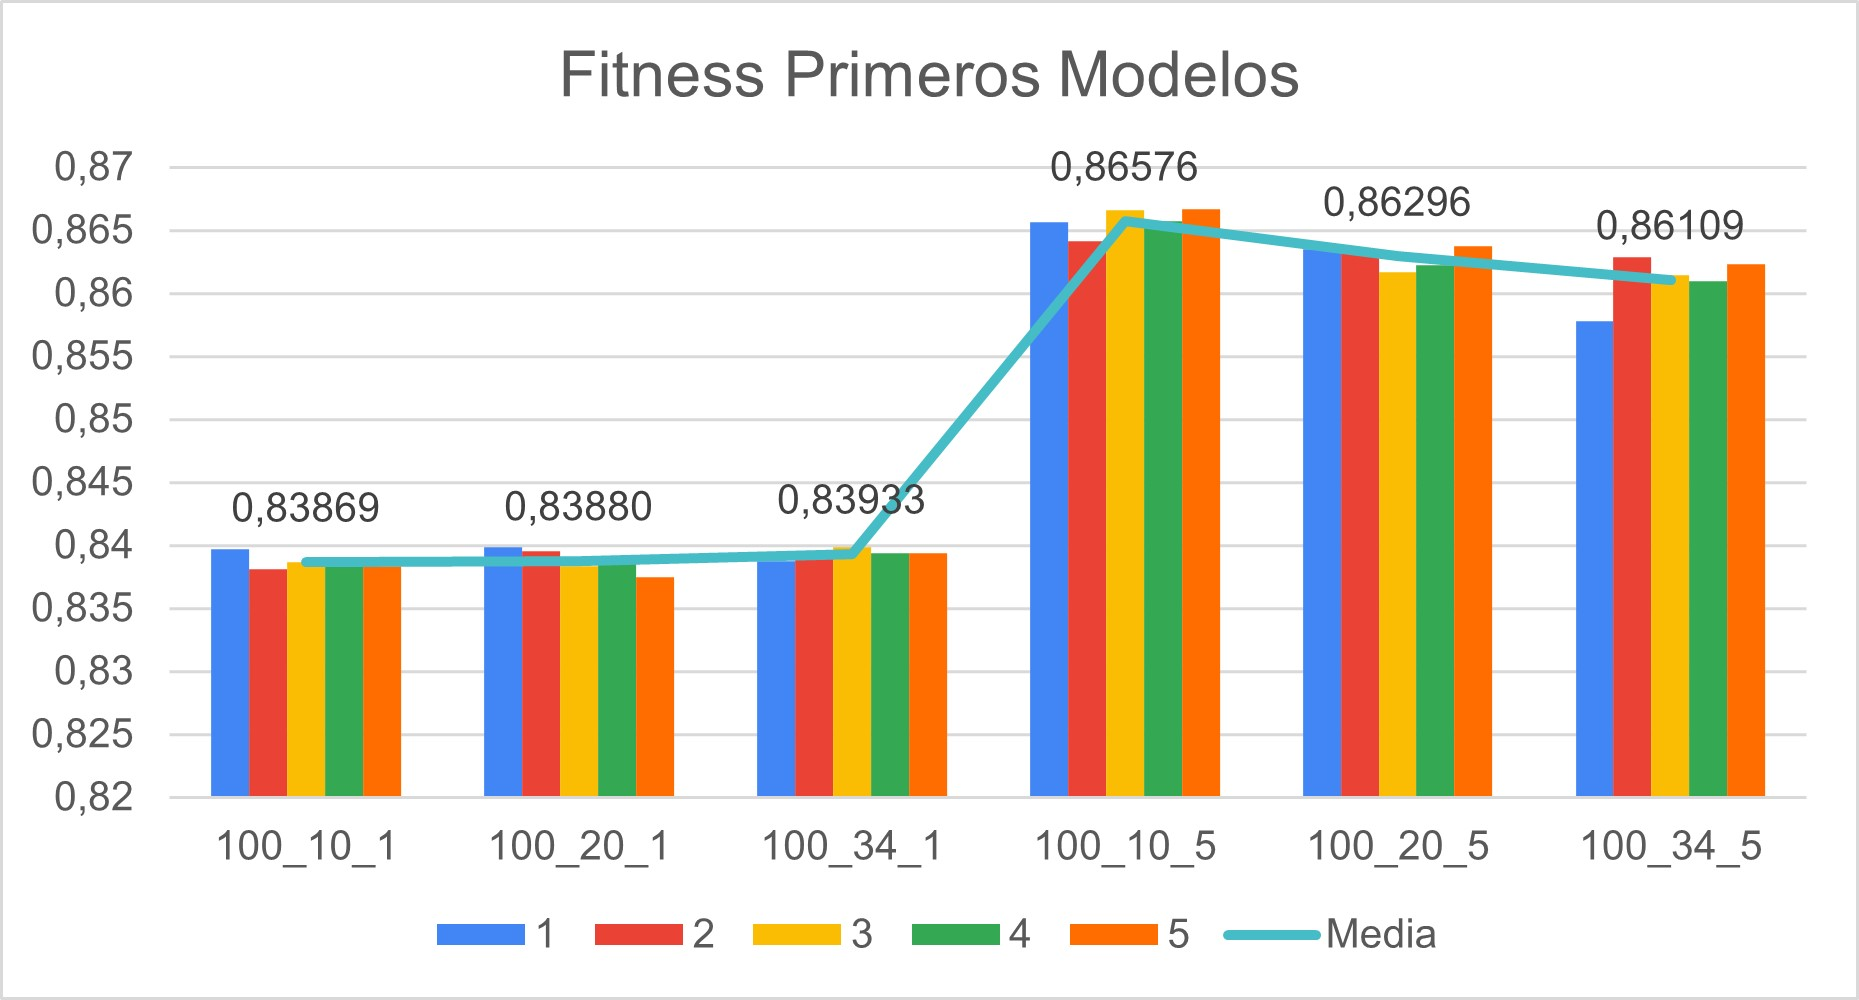
\includegraphics[scale=.8]{./img/first_models.jpg}}
\end{figure}
Los datos en los que se basa la gráfica son los de la siguiente tabla, en la que se ha marcado para cada uno de los modelos cuál es la mejor prueba en una escala de verde a rojo, siendo verde el mejor y rojo el peor. Se ha elegido el gradiente para cada modelo y no en general para facilitar la distinción de los tonos de colores. Además, se presenta la media de las pruebas, también siguiendo el gradiente de color verde a rojo.
\begin{table}[H]
	\centering
	\caption{Fitness primeros modelos}
	\resizebox{\textwidth}{!}{%
		\begin{tabular}{|l|l|l|l|l|l|l|}
			\hline
			\rowcolor[HTML]{4285F4}
			\multicolumn{1}{|c|}{\cellcolor[HTML]{4285F4}{\color[HTML]{FFFFFF} \textbf{Modelo}}} & \multicolumn{1}{c|}{\cellcolor[HTML]{4285F4}{\color[HTML]{FFFFFF} \textbf{1}}} & \multicolumn{1}{c|}{\cellcolor[HTML]{4285F4}{\color[HTML]{FFFFFF} \textbf{2}}} & \multicolumn{1}{c|}{\cellcolor[HTML]{4285F4}{\color[HTML]{FFFFFF} \textbf{3}}} & \multicolumn{1}{c|}{\cellcolor[HTML]{4285F4}{\color[HTML]{FFFFFF} \textbf{4}}} & \multicolumn{1}{c|}{\cellcolor[HTML]{4285F4}{\color[HTML]{FFFFFF} \textbf{5}}} & \multicolumn{1}{c|}{\cellcolor[HTML]{4285F4}{\color[HTML]{FFFFFF} \textbf{Media}}} \\ \hline
			100\_10\_1                                                                           & \cellcolor[HTML]{F8696B}0,839749196                                            & \cellcolor[HTML]{63BE7B}0,838089054                                            & \cellcolor[HTML]{FFE683}0,838665365                                            & \cellcolor[HTML]{FFEB84}0,838618184                                            & \cellcolor[HTML]{AAD27F}0,838332600                                            & \cellcolor[HTML]{63BE7B}0,838690880                                                \\ \hline
			100\_20\_1                                                                           & \cellcolor[HTML]{F8696B}0,839900614                                            & \cellcolor[HTML]{FB8F73}0,839552573                                            & \cellcolor[HTML]{D8DF81}0,838388457                                            & \cellcolor[HTML]{FFEB84}0,838693558                                            & \cellcolor[HTML]{63BE7B}0,837454293                                            & \cellcolor[HTML]{64BE7B}0,838797899                                                \\ \hline
			100\_34\_1                                                                           & \cellcolor[HTML]{63BE7B}0,838723301                                            & \cellcolor[HTML]{E8E482}0,839284199                                            & \cellcolor[HTML]{F8696B}0,839858925                                            & \cellcolor[HTML]{FFEB84}0,839379061                                            & \cellcolor[HTML]{FFE483}0,839406925                                            & \cellcolor[HTML]{6BC07B}0,839330482                                                \\ \hline
			100\_10\_5                                                                           & \cellcolor[HTML]{F4E783}0,865632538                                            & \cellcolor[HTML]{63BE7B}0,86411608                                             & \cellcolor[HTML]{F9766E}0,866606617                                            & \cellcolor[HTML]{FFEB84}0,865743354                                            & \cellcolor[HTML]{F8696B}0,866698111                                            & \cellcolor[HTML]{F8696B}0,865759340                                                \\ \hline
			100\_20\_5                                                                           & \cellcolor[HTML]{FFEB84}0,863509641                                            & \cellcolor[HTML]{FED680}0,863550346                                            & \cellcolor[HTML]{63BE7B}0,861678928                                            & \cellcolor[HTML]{96CC7D}0,862286523                                            & \cellcolor[HTML]{F8696B}0,863758435                                            & \cellcolor[HTML]{FA8170}0,862956774                                                \\ \hline
			100\_34\_5                                                                           & \cellcolor[HTML]{63BE7B}0,857793513                                            & \cellcolor[HTML]{F8696B}0,86290718                                             & \cellcolor[HTML]{FFEB84}0,861455499                                            & \cellcolor[HTML]{EAE582}0,860982293                                            & \cellcolor[HTML]{FB9E76}0,862319070                                            & \cellcolor[HTML]{FB9173}0,861091511                                                \\ \hline
		\end{tabular}%
	}
\end{table}
\vspace{-.5cm}
Podemos ver que en general aumentar el porcentaje de mutaciones empeora los resultados y que dentro de aquellos con un 1 \% de mutaciones, el mejor aunque no por mucho es el de menor tamaño de torneo, 10 individuos.

Hasta este punto el mejor modelo ha sido \textbf{100\_10\_1} con un \textbf{fitness de 0,838089054} en \textbf{10100 evaluaciones}, de media este modelo tarda 9320 evaluaciones en alcanzar su mejor resultado, el cromosoma que da este fitness es: 0011011100101010 1100000110101111 1010100100100001 0001010010011111 0001010010101011 1110101000101110 0001100100101011 1011010110001110 0101010110100011 0011100010100011 1110000110101000 0111010010101101 0101000000101010 1011000010001001 1111000110010011 1110000000000011 0010000010101111 1011000110001011 1001000100010011 1000100111111110 1101100010110010 0101000100011011 0100100010111101 0011000110111100. 

Se puede ver a continuación que el fitness ha ido bajando más rápido al principio y que se ha estabilizado al final por lo que las 100 generaciones han sido suficiente para que convergiera. 
\begin{figure}[H]
	\ffigbox[\FBwidth]
	{\caption{Fitness vs. Evaluaciones 100\_10\_1}}
	{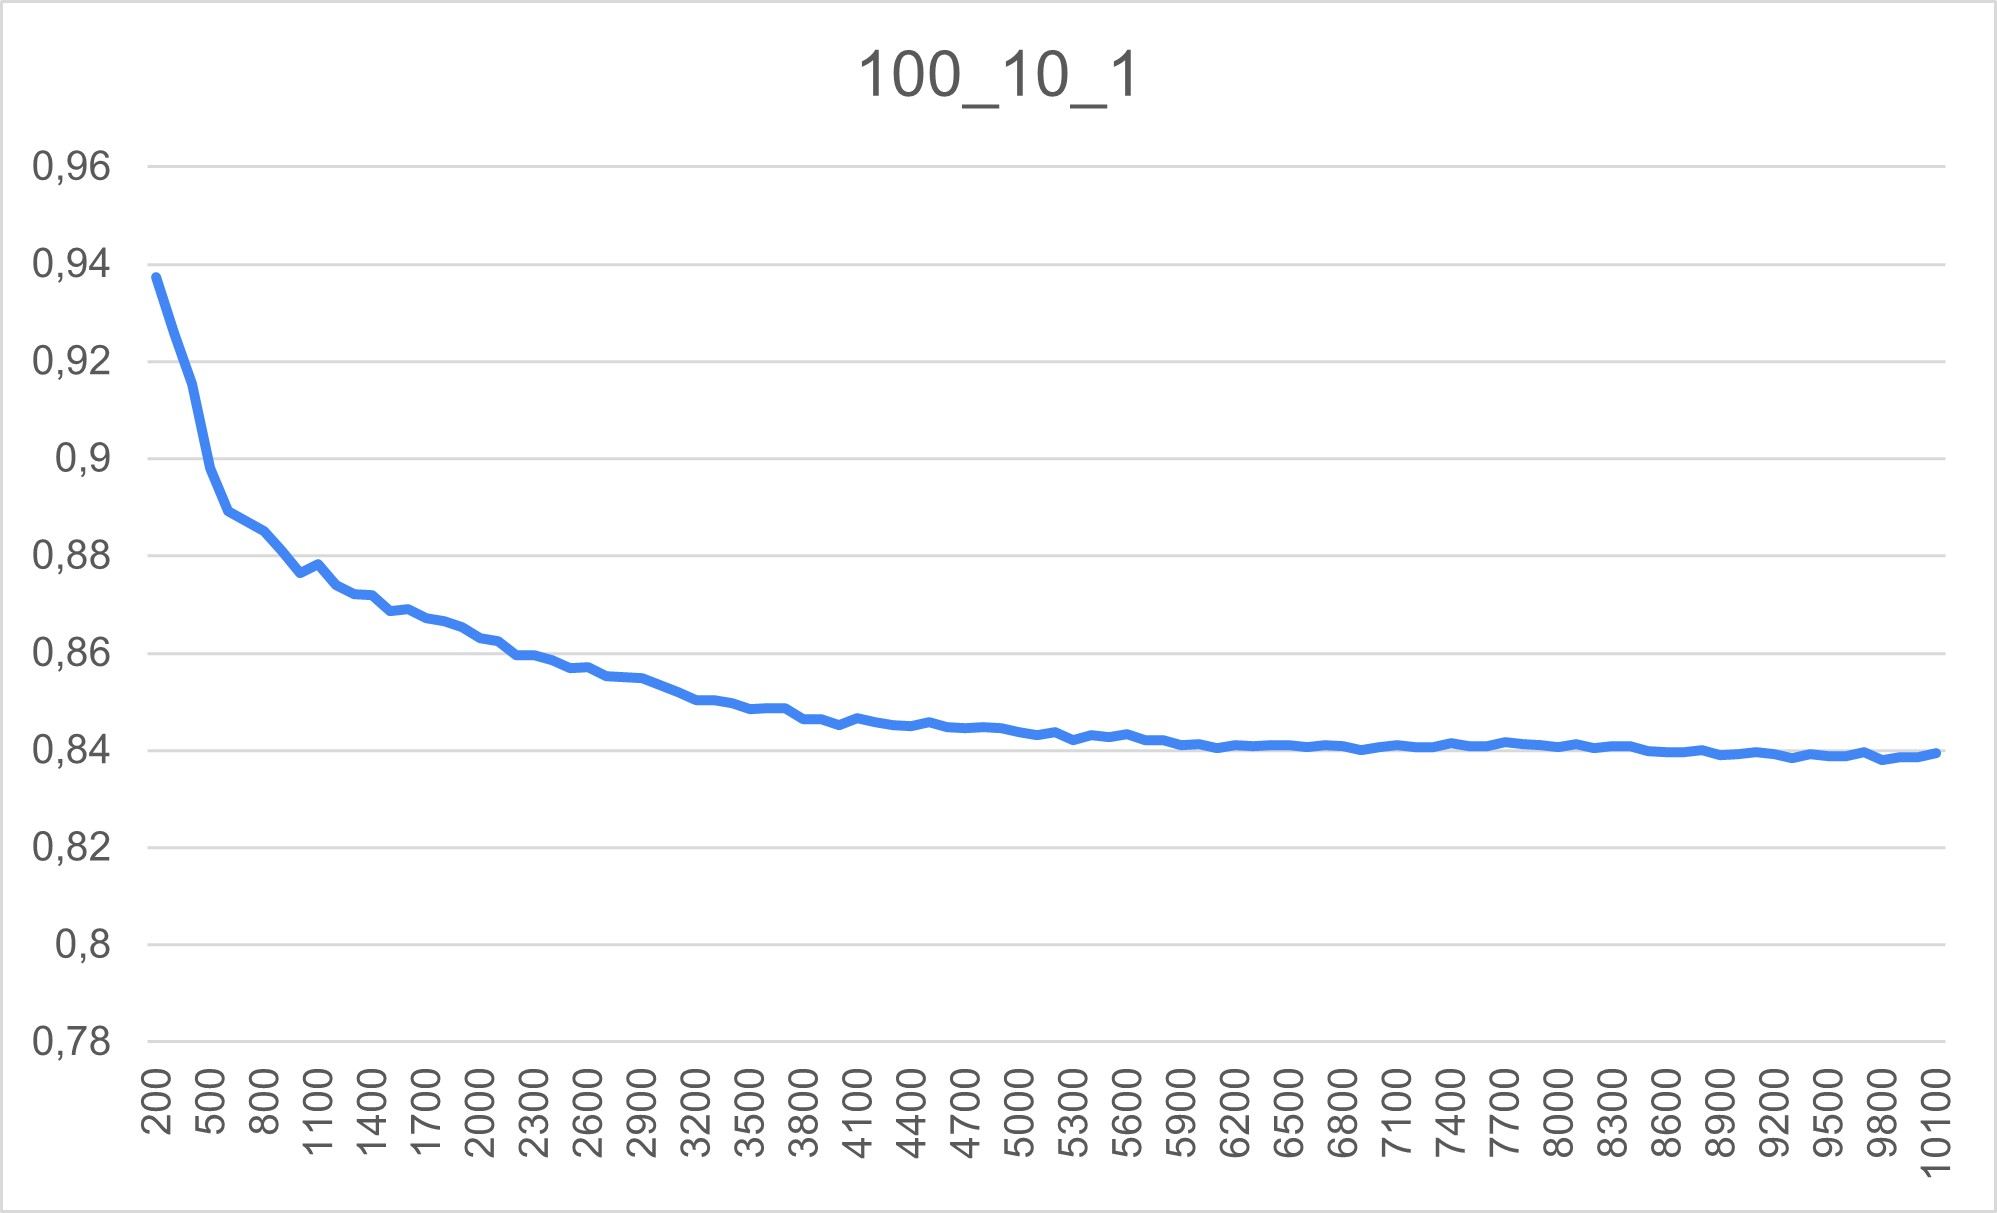
\includegraphics[scale=.75]{./img/100_10_1.jpg}}
\end{figure}

En vista de los resultados anteriores, se va a probar primero a reducir los \textbf{tamaños de torneo a 6 y 4 individuos}, se ha aumentado el número de generaciones (150) para que puedan seguir convergiendo con normalidad. En la siguiente gráfica se pueden ver los resultados nuevos comparados con los previos para un tamaño diferente de torneo:
\begin{figure}[H]
	\ffigbox[\FBwidth]
	{\caption{Pruebas Tamaño de torneo}}
	{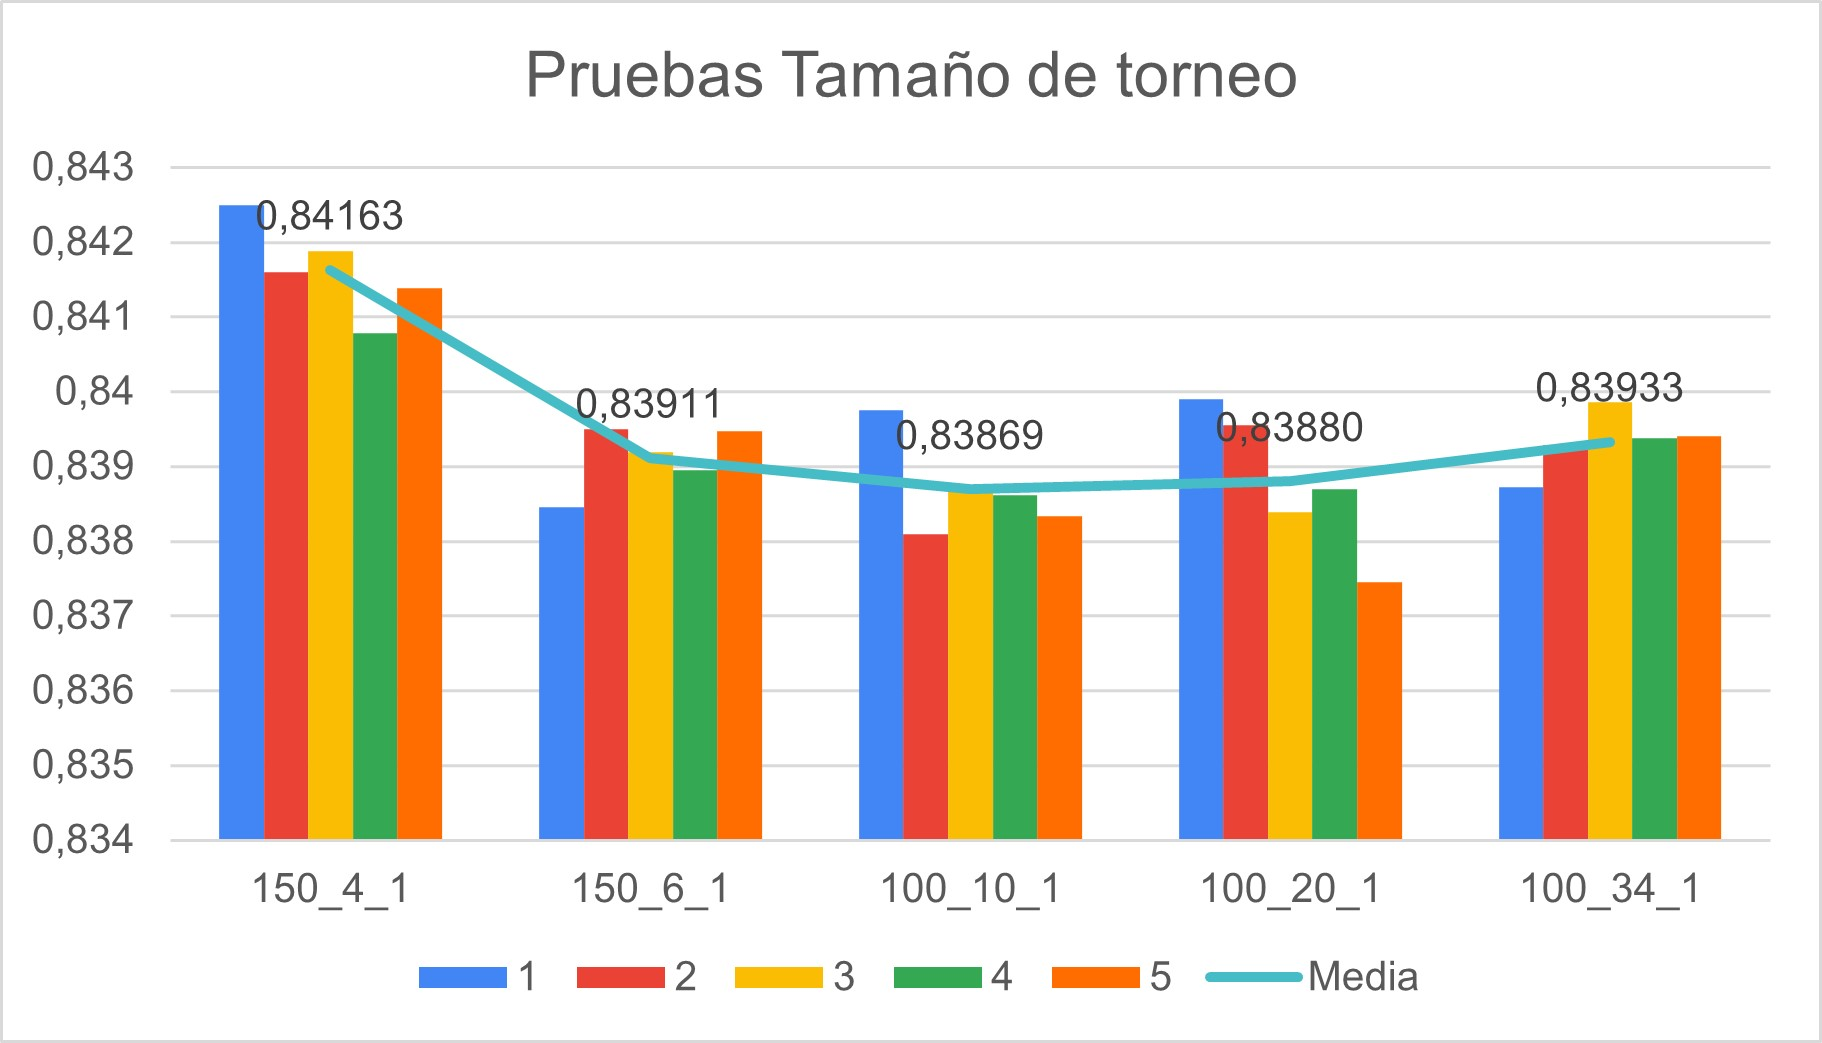
\includegraphics[scale=.8]{./img/sizes.jpg}}
\end{figure}
\begin{table}[H]
	\centering
	\caption{Resultados pruebas Tamaño de torneo}
	\resizebox{\textwidth}{!}{%
		\begin{tabular}{|l|l|l|l|l|l|l|}
			\hline
			\rowcolor[HTML]{4285F4}
			\multicolumn{1}{|c|}{\cellcolor[HTML]{4285F4}{\color[HTML]{FFFFFF} \textbf{Modelo}}} & \multicolumn{1}{c|}{\cellcolor[HTML]{4285F4}{\color[HTML]{FFFFFF} \textbf{1}}} & \multicolumn{1}{c|}{\cellcolor[HTML]{4285F4}{\color[HTML]{FFFFFF} \textbf{2}}} & \multicolumn{1}{c|}{\cellcolor[HTML]{4285F4}{\color[HTML]{FFFFFF} \textbf{3}}} & \multicolumn{1}{c|}{\cellcolor[HTML]{4285F4}{\color[HTML]{FFFFFF} \textbf{4}}} & \multicolumn{1}{c|}{\cellcolor[HTML]{4285F4}{\color[HTML]{FFFFFF} \textbf{5}}} & \multicolumn{1}{c|}{\cellcolor[HTML]{4285F4}{\color[HTML]{FFFFFF} \textbf{Media}}} \\ \hline
			150\_4\_1                                                                            & \cellcolor[HTML]{F8696B}0,842500104                                            & \cellcolor[HTML]{FFEB84}0,841600173                                            & \cellcolor[HTML]{FDC37D}0,841883423                                            & \cellcolor[HTML]{63BE7B}0,840779624                                            & \cellcolor[HTML]{D7DF81}0,841391787                                            & \cellcolor[HTML]{F8696B}0,841631022                                                \\ \hline
			150\_6\_1                                                                            & \cellcolor[HTML]{63BE7B}0,838459152                                            & \cellcolor[HTML]{F8696B}0,839499871                                            & \cellcolor[HTML]{FFEB84}0,839189223                                            & \cellcolor[HTML]{CBDC81}0,838947477                                            & \cellcolor[HTML]{F9766E}0,839470902                                            & \cellcolor[HTML]{FFEB84}0,839113325                                                \\ \hline
			100\_10\_1                                                                           & \cellcolor[HTML]{F8696B}0,839749196                                            & \cellcolor[HTML]{63BE7B}0,838089054                                            & \cellcolor[HTML]{FFE683}0,838665365                                            & \cellcolor[HTML]{FFEB84}0,838618184                                            & \cellcolor[HTML]{AAD27F}0,838332600                                            & \cellcolor[HTML]{63BE7B}0,838690880                                                \\ \hline
			100\_20\_1                                                                           & \cellcolor[HTML]{F8696B}0,839900614                                            & \cellcolor[HTML]{FB8F73}0,839552573                                            & \cellcolor[HTML]{D8DF81}0,838388457                                            & \cellcolor[HTML]{FFEB84}0,838693558                                            & \cellcolor[HTML]{63BE7B}0,837454293                                            & \cellcolor[HTML]{8AC97D}0,838797899                                                \\ \hline
			100\_34\_1                                                                           & \cellcolor[HTML]{63BE7B}0,838723301                                            & \cellcolor[HTML]{E8E482}0,839284199                                            & \cellcolor[HTML]{F8696B}0,839858925                                            & \cellcolor[HTML]{FFEB84}0,839379061                                            & \cellcolor[HTML]{FFE483}0,839406925                                            & \cellcolor[HTML]{FFE082}0,839330482                                                \\ \hline
			100\_34\_5                                                                           & \cellcolor[HTML]{63BE7B}0,857793513                                            & \cellcolor[HTML]{F8696B}0,86290718                                             & \cellcolor[HTML]{FFEB84}0,861455499                                            & \cellcolor[HTML]{EAE582}0,860982293                                            & \cellcolor[HTML]{FB9E76}0,862319070                                            & \cellcolor[HTML]{FB9173}0,861091511                                                \\ \hline
		\end{tabular}%
	}
\end{table}

Podemos apreciar que de media el mejor modelo sigue siendo 100\_10\_1, cabe mencionar que aun así el mejor resultado lo ha dado 100\_20\_1 con 0,837454293 de fitness y cromosoma 0011001100101010 1100000110111110 1010100100110001 0101000010001110 0001000010101001 1110100100100110 0001100000101111 1011010110111110 0101010110100111 0011100010100011 1110000110101000 0111000010101101 0011000000101010 1011000010101001 1101000110010011 1100001000000111 0010000010101111 1111000110001011 1001000100011011 1001110001111111 0111100010111011 0101000100110011 0100100010111100 0011000010111100. Por lo que continuaremos las pruebas con un tamaño de 10 individuos.

Ahora pasamos a buscar uno de los parámetros más importantes, el valor para la mutación, basado en la mejor prueba anterior se procede a reducir el \textbf{porcentaje de mutación a 0,5 \%, 0,1 \% y 0,05 \%}. Para estas pruebas se ha aumentado el número de generaciones, ya que en cada generación se realizan movimientos en el espacio de soluciones más pequeños y tardan más en converger. A continuación se presentan estos nuevos modelos:
\begin{figure}[H]
	\ffigbox[\FBwidth]
	{\caption{Pruebas Porcentaje de mutación}}
	{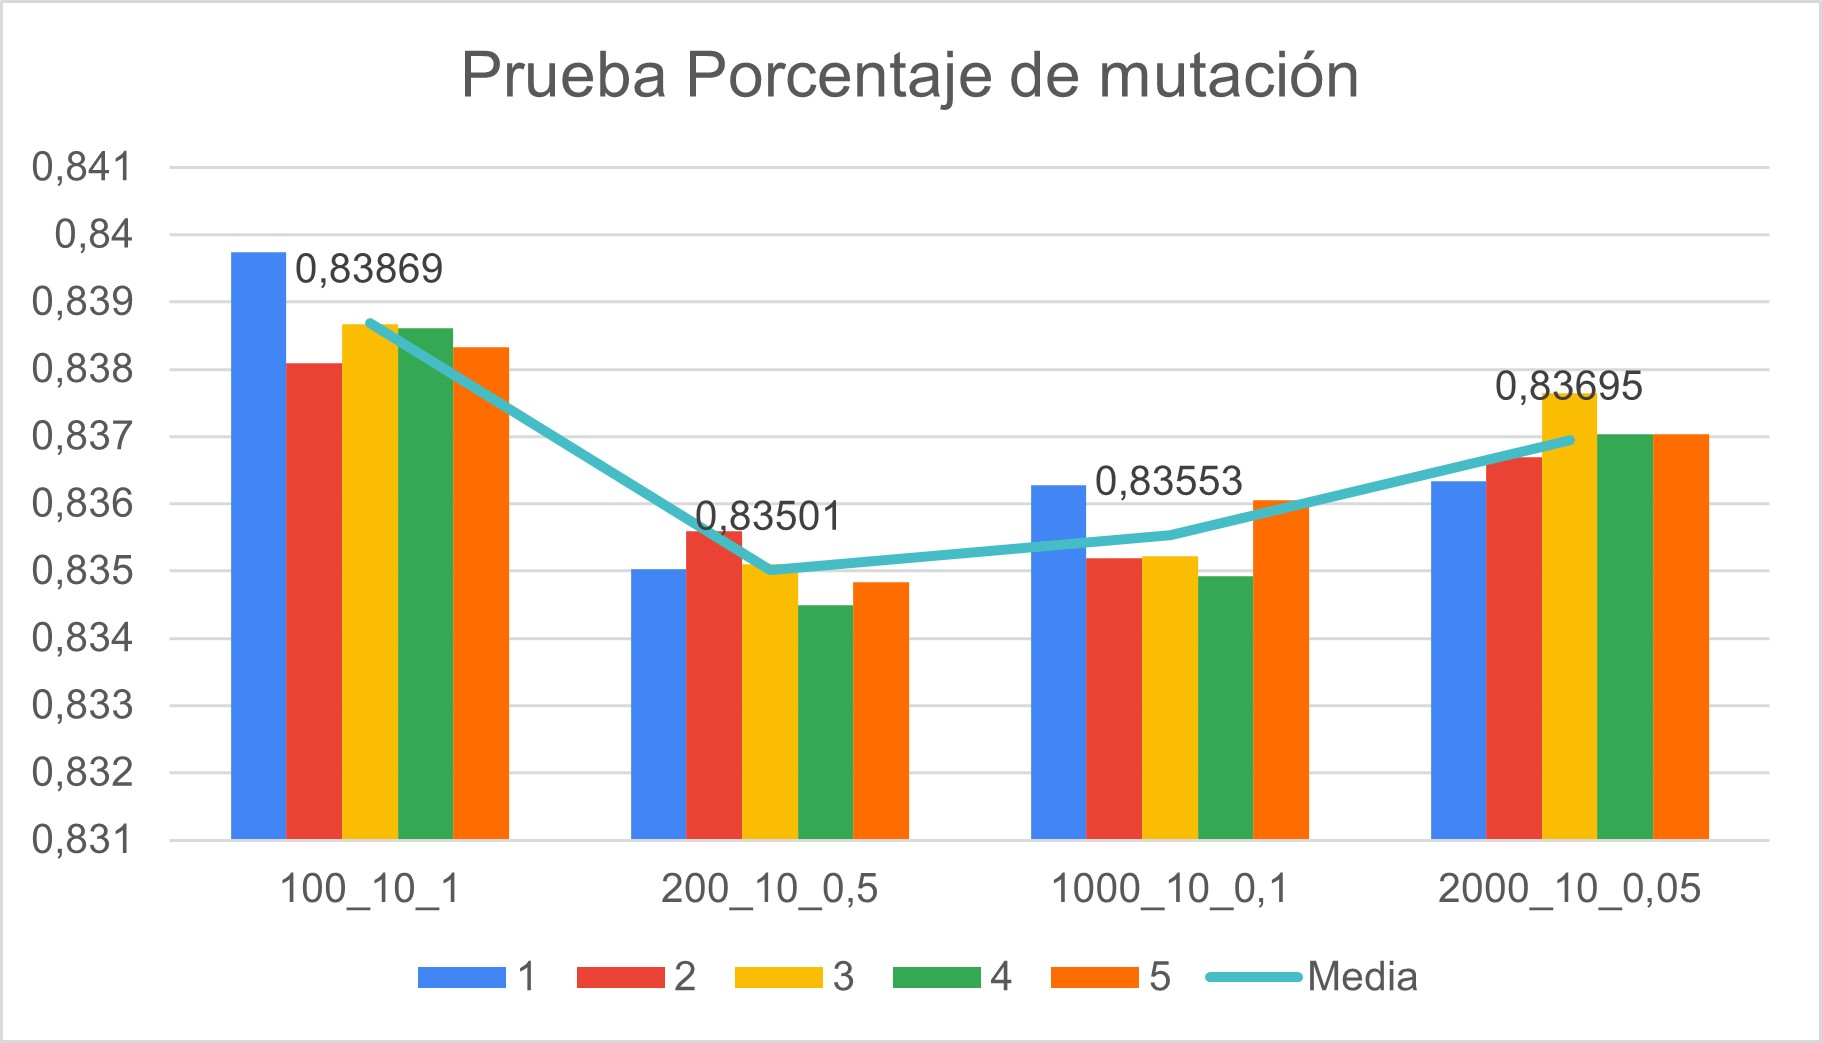
\includegraphics[scale=.8]{./img/mutation.jpg}}
\end{figure}
\begin{table}[H]
	\centering
	\caption{Resultados pruebas Porcentaje de mutación}
	\resizebox{\textwidth}{!}{%
		\begin{tabular}{|l|l|l|l|l|l|l|}
			\hline
			\rowcolor[HTML]{4285F4}
			\multicolumn{1}{|c|}{\cellcolor[HTML]{4285F4}{\color[HTML]{FFFFFF} \textbf{Modelo}}} & \multicolumn{1}{c|}{\cellcolor[HTML]{4285F4}{\color[HTML]{FFFFFF} \textbf{1}}} & \multicolumn{1}{c|}{\cellcolor[HTML]{4285F4}{\color[HTML]{FFFFFF} \textbf{2}}} & \multicolumn{1}{c|}{\cellcolor[HTML]{4285F4}{\color[HTML]{FFFFFF} \textbf{3}}} & \multicolumn{1}{c|}{\cellcolor[HTML]{4285F4}{\color[HTML]{FFFFFF} \textbf{4}}} & \multicolumn{1}{c|}{\cellcolor[HTML]{4285F4}{\color[HTML]{FFFFFF} \textbf{5}}} & \multicolumn{1}{c|}{\cellcolor[HTML]{4285F4}{\color[HTML]{FFFFFF} \textbf{Media}}} \\ \hline
			100\_10\_1                                                                           & \cellcolor[HTML]{F8696B}0,839749196                                            & \cellcolor[HTML]{63BE7B}0,838089054                                            & \cellcolor[HTML]{FFE683}0,838665365                                            & \cellcolor[HTML]{FFEB84}0,838618184                                            & \cellcolor[HTML]{AAD27F}0,838332600                                            & \cellcolor[HTML]{F8696B}0,838690880                                                \\ \hline
			200\_10\_0,5                                                                         & \cellcolor[HTML]{FFEB84}0,835029194                                            & \cellcolor[HTML]{F8696B}0,835595839                                            & \cellcolor[HTML]{FFD981}0,835107857                                            & \cellcolor[HTML]{63BE7B}0,834496455                                            & \cellcolor[HTML]{C6DA80}0,834835753                                            & \cellcolor[HTML]{63BE7B}0,835013020                                                \\ \hline
			1000\_10\_0,1                                                                        & \cellcolor[HTML]{F8696B}0,836276467                                            & \cellcolor[HTML]{ECE582}0,835187671                                            & \cellcolor[HTML]{FFEB84}0,835223458                                            & \cellcolor[HTML]{63BE7B}0,834919949                                            & \cellcolor[HTML]{FA8471}0,836060705                                            & \cellcolor[HTML]{A5D17E}0,835533650                                                \\ \hline
			2000\_10\_0,05                                                                       & \cellcolor[HTML]{63BE7B}0,836333763                                            & \cellcolor[HTML]{B1D47F}0,836686695                                            & \cellcolor[HTML]{F8696B}0,837647729                                            & \cellcolor[HTML]{FFEB84}0,83703896                                             & \cellcolor[HTML]{FFEB84}0,837036178                                            & \cellcolor[HTML]{FDC67D}0,836948665                                                \\ \hline
		\end{tabular}%
	}
\end{table}

Como podemos ver hemos conseguido mejorar el modelo previo reduciendo el porcentaje de mutación, los 3 nuevos modelos son mejores. Estos resultados han sido favorables, puesto que una vez encontrado el tamaño de torneo que favorece que se escojan los mejores individuos, solo nos quedaba ajustar en qué medida debían ir cambiando los cromosomas, de manera que no dieran grandes saltos en el espacio de soluciones, pero tampoco como para que se estancase en resultados subóptimos. En ninguno de los casos se ha estancado el modelo, aun dándoles muchas generaciones.

El nuevo \textbf{mejor modelo es 200\_10\_0,5} con un fitness de 0,834496454567, tarda de media 18140 evaluaciones en alcanzar su mejor evaluación, en la siguiente sección se profundizará, pero a continuación el progreso del fitness a lo largo de las evaluaciones.

\begin{figure}[H]
	\ffigbox[\FBwidth]
	{\caption{Fitness vs. Evaluaciones 200\_10\_0,5}}
	{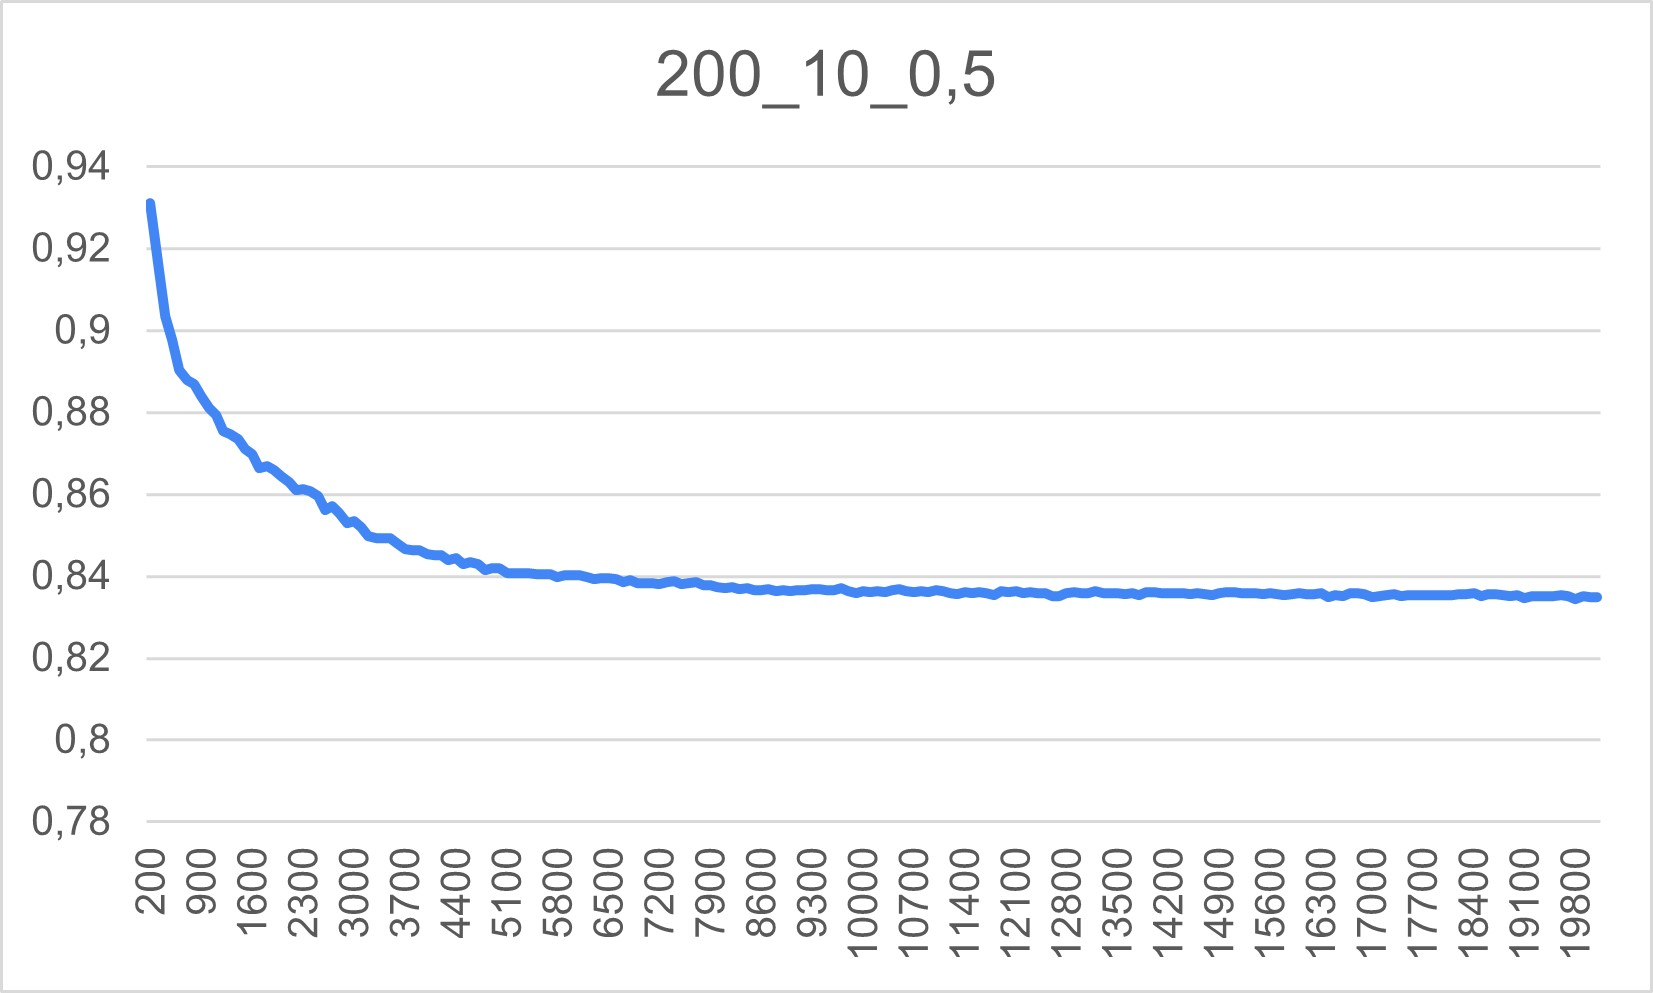
\includegraphics[scale=.8]{./img/200_10_0,5.jpg}}
\end{figure}

\subsection{Resultado}
El mejor modelo que hemos llegado a obtener ha sido el \textbf{200\_10\_0,5}, que corresponde a \textbf{200 generaciones} que han sido \textbf{20100 evaluaciones} con un tamaño de \textbf{torneo de 10 individuos} y un porcentaje de \textbf{mutación del 0,5 \%} de la población, el resultado obtenido tiene un \textbf{fitness de 0,834496454567} y su cromosoma asociado es:

0011010100101011 1100000110111111 1010100100101001 0101000010011110 0001000010101011 1100001010001110 0001000110101101 1011000110111110 0101010110100011 0011100000000111 1110000110101000 0111000010101101 0111000000101010 1011000010001001 1101000110010011 1110000000011011 0010000010101111 0011000010001111 1001000100010011 1001110001111110 1111100010110011 0101000100010011 0100100010111100 0011000010111100
\pagebreak

El significado de este cromosoma es que las estaciones tendrán los siguientes sensores:
\begin{itemize}
	\item \textbf{Estación 1:} NO, NO$_2$, PM10, O$_3$, EBE, PXY, TCH y NMHC.
	\item \textbf{Estación 2:} SO$_2$, CO, O$_3$, TOL, EBE, MXY, PXY, OXY, TCH y NMHC.
	\item \textbf{Estación 3:} SO$_2$, NO, PM2.5, O$_3$, EBE, PXY y NMHC.
	\item \textbf{Estación 4:} CO, NO$_2$, TOL, MXY, PXY, OXY y TCH.
	\item \textbf{Estación 5:} NO$_2$, TOL, EBE, PXY, TCH y NMHC.
	\item \textbf{Estación 6:} SO$_2$, CO, NOx, TOL, PXY, OXY y TCH.
	\item \textbf{Estación 7:} NO$_2$, O$_3$, TOL, EBE, PXY, OXY y NMHC.
	\item \textbf{Estación 8:} SO$_2$, NO, NO$_2$, O$_3$, TOL, EBE, MXY, PXY, OXY y TCH.
	\item \textbf{Estación 9:} CO, NO$_2$, PM10, O$_3$, TOL, EBE, TCH y NMHC.
	\item \textbf{Estación 10:} NO, NO$_2$, PM2.5, OXY, TCH y NMHC.
	\item \textbf{Estación 11:} SO$_2$, CO, NO, O$_3$, TOL, EBE y PXY.
	\item \textbf{Estación 12:} CO, NO, NO$_2$, TOL, EBE, PXY, OXY y NMHC.
	\item \textbf{Estación 13:} CO, NO, NO$_2$, EBE, PXY y TCH.
	\item \textbf{Estación 14:} SO$_2$, NO, NO$_2$, TOL, PXY y NMHC.
	\item \textbf{Estación 15:} SO$_2$, CO, NO$_2$, O$_3$, TOL, MXY, TCH y NMHC.
	\item \textbf{Estación 16:} SO$_2$, CO, NO, MXY, PXY, TCH y NMHC.
	\item \textbf{Estación 17:} NO, TOL, EBE, PXY, OXY, TCH y NMHC.
	\item \textbf{Estación 18:} NO, NO$_2$, TOL, PXY, OXY, TCH y NMHC.
	\item \textbf{Estación 19:} SO$_2$, NO$_2$, O$_3$, MXY, TCH y NMHC.
	\item \textbf{Estación 20:} SO$_2$, NO$_2$, PM2.5, PM10, BEN, EBE, MXY, PXY, OXY y TCH.
	\item \textbf{Estación 21:} SO$_2$, CO, NO, NO$_2$, PM2.5, TOL, EBE, MXY, TCH y NMHC.
	\item \textbf{Estación 22:} CO, NO$_2$, O$_3$, MXY, TCH y NMHC.
	\item \textbf{Estación 23:} CO, PM2.5, TOL, EBE, MXY, PXY y OXY.
	\item \textbf{Estación 24:} NO, NO$_2$, TOL, EBE, MXY, PXY y OXY.
\end{itemize}

\section{Conclusiones}
En este proyecto se ha abordado el problema de seleccionar sensores para estaciones de control de calidad del aire en la ciudad Madrid, desde dos enfoques, uno clásico como es la búsqueda por fuerza bruta y otro con computación evolutiva mediante algoritmos genéticos. Se ha podido comprobar que el enfoque clásico se ve muy limitado por la gran cantidad de tiempo que se necesita para realizarlo, por lo que la computación evolutiva ha resultado ser el método más práctico y rápido, ya que entre la prácticamente infinita cantidad de posibilidades que existen es capaz de encontrar una solución suficientemente adecuada.

\end{document}